\documentclass{article}

\usepackage[utf8]{inputenc}

\usepackage{graphicx}
\graphicspath{{images/}}

\renewcommand{\familydefault}{\sfdefault}
\usepackage[a4paper]{geometry}

\usepackage{listings}
\lstset{language=SQL}

\usepackage{tcolorbox}
\newtcolorbox{keypointbox}
{
    arc=0mm,
    colback=red!20,
    colframe=red!80,
    leftrule=5pt,
    toprule=0pt,
    rightrule=0pt,
    bottomrule=0pt
}

\setcounter{secnumdepth}{2}

\usepackage{hyperref}
\usepackage{cleveref}

\title{Data Warehouse Systems}
\author{Alexander Schlögl}

\begin{document}
\maketitle
\section{Definition}
\textbf{GI-Group Definition:}
“A Data Warehouse is a database which (from a technical point of view) integrates data from different (heterogeneous) data sources and (from an economic point of view) provides the user with this data for business analysis purposes. Frequently, but not necessarily, a historization of data takes place.”
\\
\textbf{Inman's Definition:}
“A data warehouse is a subject-oriented, integrated, time-variant and non-volatile collection of data in support of management's decision making process.”
\textbf{Integrated} means the data is collected from multiple (separate) sources, and compiled into a single source of truth.
\textbf{Time-variant} means that the data is accurate at the time it was compiled (ie. the transactions took place).
This is very useful for observing changing trends.
\textbf{Non-volatile} means the compiled data in the DWS is not changed (often), but only queried.
\begin{keypointbox}
    A DWS is a static copy of accumulated transaction data used for analysis.
\end{keypointbox}

Data Warehouses are not single products, but a system comprised of multiple interacting components, most of which are usually bought from third-parties.

\subsection{Operational Data Stores vs. Data Warehouses}
Operational Data Stores (ODSs) are used in the day to day transactions of a business.
They are very fast, use a single data source, are used by multiple users concurrently and mostly perform small transactions (e.g. sales).
Think of the database interacting with Point of Sale terminals in a supermarket.

Data Warehouse (DWs) are very large databases used to store accumulated data.
They are usually only accessed by single users and even then mostly only for reads.
Data is fed into DWs periodically (e.g. daily or weekly), and then usually not changed afterwards.
This means that locks can be optimized differently for DWs than for ODSs.
The access patterns are also very different from ODSs, with range queries being the norm.

A full comparison is given in \Cref{tbl:odsDwComp}.

\begin{table}[ht]
    \center
    \begin{tabular}{| l | l | l |}
        \hline
        & ODS & DW\\
        \hline
        Data Sources & mostly only one & many\\
        Data Volume & MB-GB & GB-TB-PB\\
        Access & Single Tuple accesses & Range queries\\
        Up-to-dateness & Up to date & (Possibly) outdated\\
        Use & Input output by employees & Evaluation by analysts/managers\\
        Number of users & Many & few\\
        Response time & ms-s & s-min-h\\
        \hline
    \end{tabular}
    \caption{Comparison between ODSs and DWs}
    \label{tbl:odsDwComp}
\end{table}

\begin{keypointbox}
    ODSs are regular databases.
    DWs are larger, and optimized for range-queries and rare modifications.
\end{keypointbox}

\begin{keypointbox}
    ODSs are used for Online Transaction Processing (OLTP), and DWs for Online Analytics Processing (OLAP).
\end{keypointbox}

\section{Reference Architecture}
\label{architecture}
The goal of a reference architecture is to provide a fundamental, abstract, implementation independent visualization of the DW.
It is useful for comparing DW models, systems and components and can be used for planning specifications and implementations of a DW system.
A reference architecture should provide an overview of the operators (functions) and operands (databases, data), as well as the \textbf{data-flow} required for the functions and the \textbf{control-flow} required for the underlying processes.

\begin{keypointbox}
    A reference architecture is a model of a DW system.
\end{keypointbox}

\subsection{Requirements of a DW architecture:}
\begin{itemize}
    \item \textbf{Isolation:} the DW should be independent of its data sources after the data has been imported.
    \item \textbf{Persistency:} after importing the data the DW should suffice as a permanent storage
    \item \textbf{Flexibility of use:} arbitrary evaluations should be possible
    \item \textbf{Scalability:} it should be easy to integrate new data sources over time
    \item \textbf{Efficiency:} repeating tasks should be easy to automate
    \item \textbf{Uniqueness} of data structures, access rights and processes
    \item \textbf{Orientation} of the system towards the analysis of data (ie. optimizations for range queries)
\end{itemize}

\subsection{Static View of a DW Architecture}
This is a view of the static components themselves, ie. the databases or the component extracting data from data sources.
The system components include:
\begin{itemize}
    \item \textbf{Interface components:} DW manager, Metadata manager
    \item \textbf{Databases:} DW, Base DB, Metadata DB
    \item \textbf{Functional components:} Monitor, Extraction, Transformation, Loading and Analysis components
\end{itemize}

The static view is (somewhat) equivalent to the white blobs in \Cref{fig:flow}.

\subsection{Dynamic View of a DW Architecture}
The dynamic view contains the data flow (comprised of main- and metadata flow) as well as the control flow.
It is depicted by the arrows in \Cref{fig:flow}, with the solid arrows being data-flow and the dashed arrows being control-flow.

\begin{figure}
    \center
    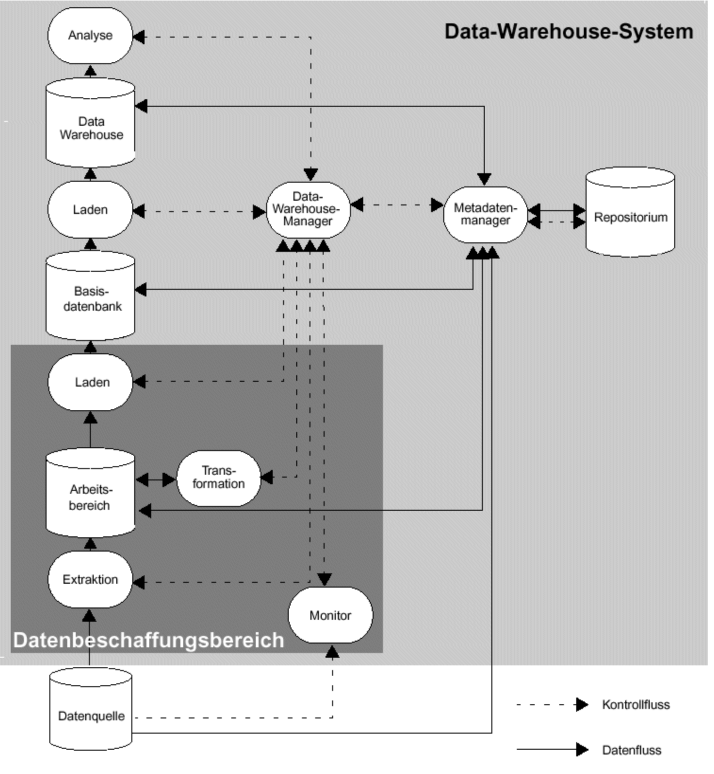
\includegraphics[width=0.8\textwidth]{control_flow.png}
    \caption{The data and control flow from a data source to the DW}
    \label{fig:flow}
\end{figure}

\subsection{Components of a DW System}
\begin{keypointbox}
    All the DW components do exactly what their name suggests.
    \Cref{fig:flow} is in principle enough to fully understand \Cref{architecture}.
\end{keypointbox}

The \textbf{monitor} handles the extraction from the data source(s), sometimes filtering out irrelevant data.
Relevant data is extracted into the (temporary) \textbf{working area}, where it is \textit{transformed} (cleaned, integrated, etc.).
To reduce potential consistency issues caused by changing dimension data (e.g. product names changing), the data can then be loaded into a \textbf{base database}.
This database contains the raw transformed data, which needs to be combined with metadata to be meaningful.
The base database is application independent and modelled based on the relations in the data.
Finally, the data can be combined with metadata and loaded into the \textbf{data warehouse} which is modelled specifically for the application (analysis).
The metadata is kept in a separate metadata \textbf{repository}.

\subsection{Data Sources}
The selection of data sources for the data warehouse is a defining factor for the quality of the finished data warehouse.
Sources must be selected based on their \textbf{relevance} and the \textbf{quality of their data}.
Factors for relevance are:
\begin{itemize}
    \item Purpose of the data warehouse
    \item Availability of the source data (technical, organisational, legal)
    \item Cost of acquisition
\end{itemize}
Factors for quality are:
\begin{itemize}
    \item Correctness
    \item Consistency
    \item Completeness
    \item Comprehensability (Metadata, documentation)
\end{itemize}

Data sources can also be classified based on a number of characteristics; examples include origin, time, usage (metadata, base-data), ...

\subsection{Control Components}
Important control components are:

The \textbf{data warehouse manager} handles initialization, control and management of all functions and other components.
It is the main control component and manages the entire work- and data-flow.

The \textbf{metadata manager} does exactly what the name says.
It manages metadata, including start and end dates of validity (important for renames and the like) and links between the data warehouse manager and the metadata repository.

\textbf{Monitors} are used (one per data source) to monitor for updates and extract new data.
They can either directly feed relevant data to the work area, or simply notify the manager of updates and wait for scheduled extraction.
Techniques for extracting are \textit{trigger-based} (periodically, ...), \textit{replication-based} (store changed tuples in special relation), \textit{timestamp-based}, \textit{log-based}, \textit{snapshot-based} (operate on deltas, high implementation effort but sometimes only possibility for legacy systems).

\subsection{Work Area}
It is a temporary storage area required for the process of data transformation, and the central storage for \textbf{ETL-components}.

\subsection{ETL-Components}
ETL stands for extraction, transformation and loading, and describes the components needed in order to fill the data warehouse with data originally from the data sources.
As the data sources are heterogeneous (e.g. different currencies, incosistent schemas, ...) the data needs to be cleaned and annotated with metadata in order to be useful.
This cleanup is done in the ETL process.

\subsubsection{Extraction Component}
Controls the periodical transmission of source data to the working area.
The extraction time determines the analysis accuracy and depends on the analysis goals.
Examples for times the extraction can take place are:
\begin{itemize}
    \item periodical
    \item on demand
    \item event-driven
    \item immediately on updates
\end{itemize}
The extraction strategy dictates the extraction techniques.

\subsubsection{Transformation Component}
Transformation is the process of reshaping the schema (column names, ...) as well as cleaning the data and unifying data types, currencies, unit formats (times, ...) etc.

During this process the data is also checked for integrity violation, illegal values (consistency and plausibility checks), redundancy, incomprehensible and inconsistent values, as well as missing and NULL values.
All these checks are part of the code cleanup.

The schema transformation that is done by this component is necessary due to a heterogenity of the data sources.
Because different data sources have different views, legal requirements or simply different models their schemas can vary wildly.
Schema transformation requires expert knowledge and is hard to automate, as a transformation script has to be created for every single data source.
It also requires the setup of the metadata database.

\Cref{fig:transformation} shows the individual steps of the transformation process.

\begin{figure}[hp]
    \centering
    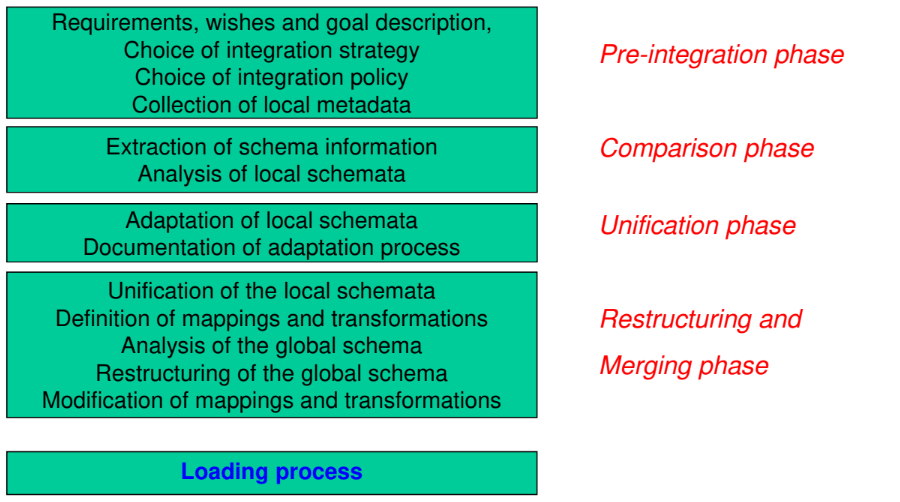
\includegraphics[width=0.8\textwidth]{transformation.png}
    \caption{The steps of the transformation process}
    \label{fig:transformation}
\end{figure}

\subsubsection{Loading Component}
This component takes care of loading the transformed data into the database(s).
If there is no base database the analytics specific data is transmitted to the data warehouse from the working area.
If such a database does exist, the cleaned data is loaded into it, and a version of the data made specifically for analysis is sent to the data warehouse.
The anlysis version might include pre-aggregated results.

\subsection{Base Database}
The base database acts as a \textbf{central data storage}.
It stores the cleaned data at the highest resolution (lowest granularity) while staying completely application netral.
It functions as a buffer between the data sources and data warehouses.

In a situation where there are multiple DWs the base database functions as the \textbf{single source of truth}, thus saving the DWs from gathering their data from each data source themselves.
This reduces complexity from $\mathcal O (m \cdot n)$ to $\mathcal O (m + n)$.

The documentation of the base database must ensure traceability for the entire data flow from the sources to the base database.
This includes the ETL process and points of possible human intervention in case the automated system fails.
The documentation of the ETL processes must be \textbf{exact} so they can be reproduced in the next iteration.

The metadata repository as well as the base database must be \textbf{available} for the DWs to function properly if they are the single source of truth.

\subsection{Data Warehouse}
The DW is specifically organized for analysis.
This includes ordering along multiple dimensions.
In order to speed up this sorting, DWs have moved to multi-dimensional representations of their data.

Special requirements for a database management system (DBMS) of a DW include:
\begin{itemize}
    \item bulk loading
    \item access interface for analysis tools
    \item Optimization and tuning for frequent queries (indices, materialized views, ...)
\end{itemize}

\subsection{Data Marts}
Data marts provide a partial view of the DW.
They can either access the DW for data (requiring a permanent connection) or save their relevant part themselves.
Both variants come with a tradeoff of availability versus integrity.

Splitting the DW into multiple data marts allows departments to operate independent of each other, as well as distributing the workload and required storage.

Data marts can be categorized by geography, organisation or function.
While they can be kept independent from the main DW by gathering the data directly after the ETL process, this causes a lot of integrity problems and \textbf{should be avoided}.

\subsection{Metadata Repository}
The metadata repository contains a description of the \textbf{entire} DW system.
This includes information about schemata, data-types, formats, but also the setup, maintenance and adminstration of the DWS itself.
It is vital for understanding the data, and without it, the base database is essentially worthless.

The repository is managed by the metadata manager component.

\subsection{Analysis tools}
Analysis tools are also called Business Intelligence (BI) tools, and operate on the DW.
They can be classified by their intended use into reporting tools, OLAP tools (used for interactive data analysis), and data mining tools (used for finding patterns in the data).

\subsubsection{OLAP systems}
These systems are used for online analytics.
Cobb (inventor of database management), defines twelve rules for a good OLAP system, which are extended in the lecture slides to 18:
\begin{enumerate}
    \item Conceptional multi-dimensional view
    \item Transparency for access from multiple data sources (Transparency in this case means that the extra steps taken for the access to a different data source are invisible (transparent) to the user, not that the access is easy to understand)
    \item Flexible access possibilities
    \item Same response time in report creation (in regard to queries on different dimensions)
    \item Client-Server architecture
    \item Equality of dimensions
    \item Adaptive administration of sparse data cubes
    \item Multi-user operation
    \item Unlimited, cross-dimensional operations
    \item Intuitive data handling
    \item Flexible reporting
    \item Unlimited number of dimensions/aggregation levels
    \item Easy data integration
    \item Support of different analysis models
    \item Separation of analysis and operative data
    \item Separation of storage areas
    \item Differentiation between NULL and non-existant values
    \item Handling of missing values
\end{enumerate}

\section{Multi-dimensional Data Modeling}
As we usually want aggregations along multiple dimensions in DWSs, we want our (conceptual) model to represent this.
Therefore we need to adapt existing modeling methods for multiple dimensions.
While our representation of the data is multi-dimensional, internally all data is still stored in relational databases, so our adapted modeling methods are very related to traditional relational modeling methods.
A comparison can be found in \Cref{fig:modeling}.

\begin{figure}[h]
    \centering
    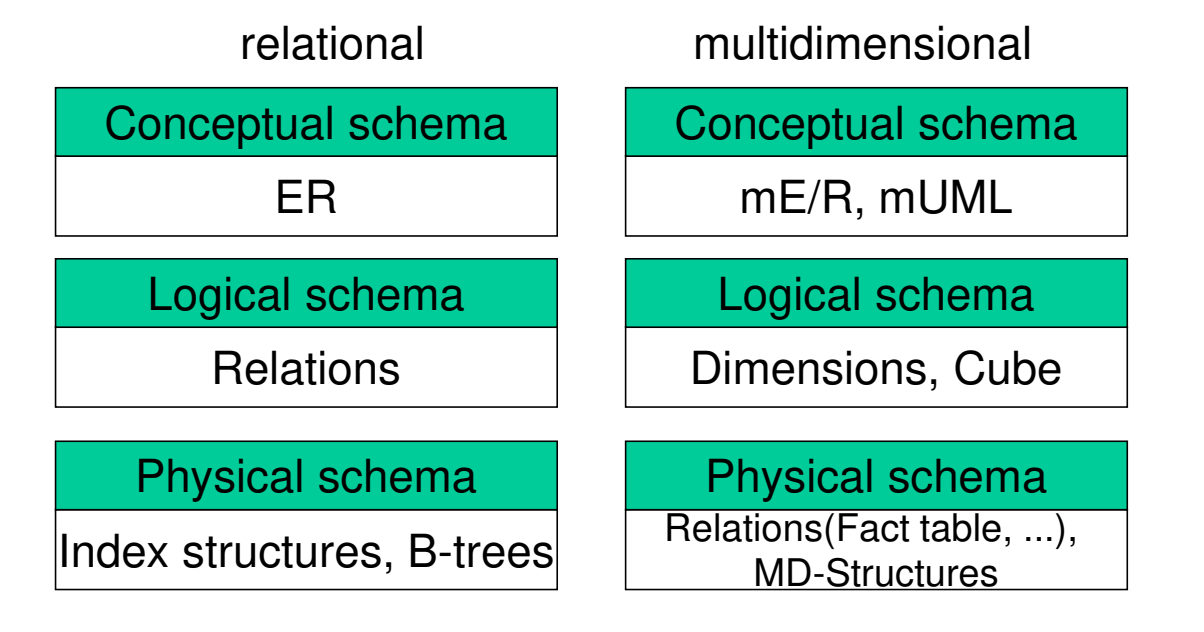
\includegraphics[width=0.6\textwidth]{modeling.png}
    \caption{A comparison of relational and multi-dimensional modeling methods}
    \label{fig:modeling}
\end{figure}

\begin{keypointbox}
    Multi-dimensional modeling works just like regular modeling.
    If you understand ER diagrams, creating mER diagrams is easy, just add multiple hierarchies.
    An example can be found in \Cref{fig:schema}.
\end{keypointbox}

\subsection{Schemas and Instances}
A classification schema (of a dimension) is a set $D$ of classification levels: $(\{D_0, ..., D_{top}\}, \rightarrow)$.
Together with their dependency operator $\rightarrow$ they become a partially ordered set (the partial order allows for multiple parallel hierarchies).
Dimension elements are occurences of the lowest classification level $D_0$ and occurences of higher classification levels are hierarchy nodes.
Three examples for a classification schema can be found in \Cref{fig:schema}.
Every path from $D_0$ to $D_{top}$ defines a classification hierarchy, and a instance of a dimension is the set of all classification hierarchies.

\begin{figure}[h]
    \centering
    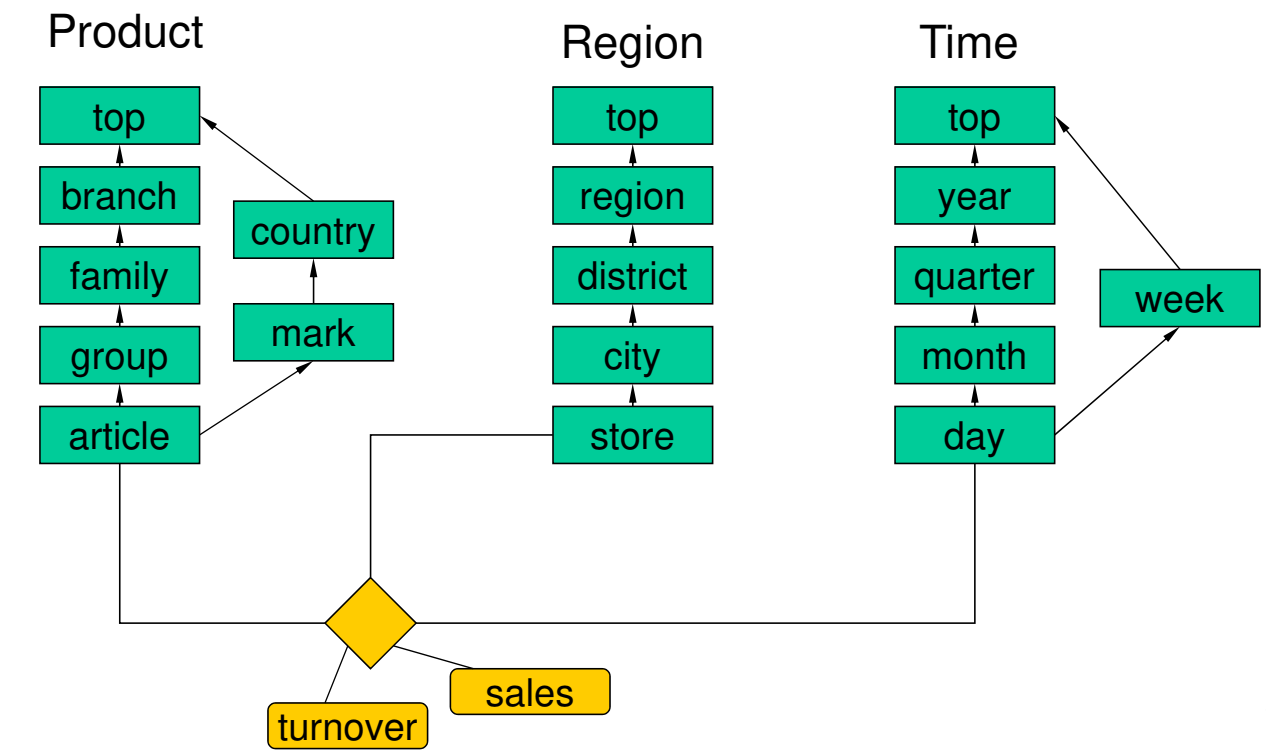
\includegraphics[width=0.8\textwidth]{schema.png}
    \caption{An example for a mER diagram with multiple classification schemes}
    \label{fig:schema}
\end{figure}

\subsection{Data cubes}
As the highest number of dimensions we can easily visualize as a geometrical shape is three, data cubes are a common representation of higher-dimensional data.
The cube consists of data cells which contain $1$ to $n$ measures, and the location in the cube along its three axes represents the values along three dimensions (e.g. geographical, time and product).

\subsubsection{Cube Schemas and Instances}
A cube schema $W\left[G,M\right]$ consists of the granularity $G$ and the set of measures $M$.
For example, if we were to store the sales of an article per store and per day, $G$ would be the set of article, store and day.
Our measures $M$ would be the sales and maybe additionally the turnover.

An instance of a cube $W$ contains all cells from the definition domain of the cube $W = dom(G) \times dom(M)$.
In general, not all cells have a value.
\Cref{fig:cube} shows an instance of a cube including classification hierarchies.

\begin{figure}[h]
    \centering
    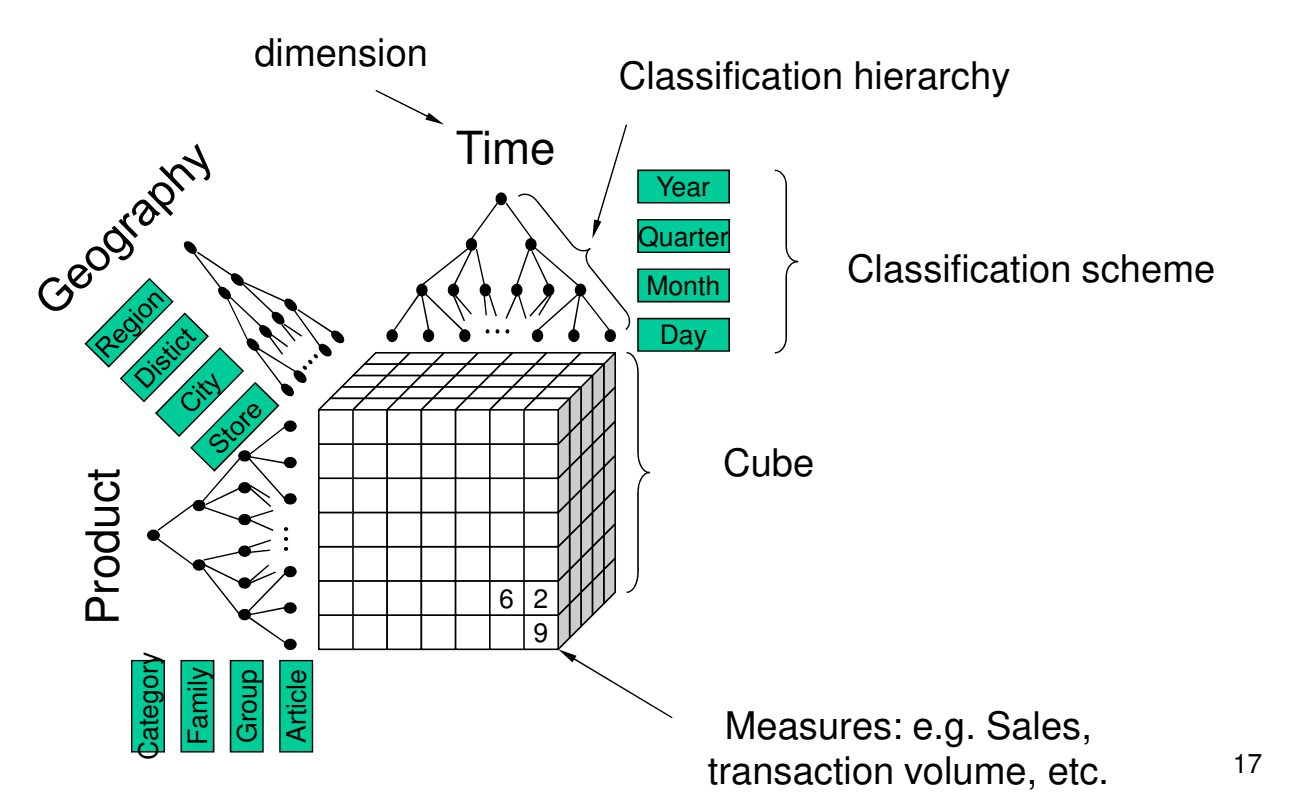
\includegraphics[width=0.8\textwidth]{cube.png}
    \caption{An instance of a data cube}
    \label{fig:cube}
\end{figure}

\subsubsection{Features of Measures}
Measures have a name, domain and aggregation type.
The domain is roughly equivalent to their data type, but restrictions are possible (e.g. negative cost).

Aggregation types are:
\begin{itemize}
    \item \textbf{FLOW:} arbitrarily aggregationable (Turnover, Sales)
    \item \textbf{STOCK:} not temporally summable (Stock)
    \item \textbf{Value per unit (VPU):} not summable (Price, taxes)
\end{itemize}

\subsubsection{Multi-dimensional Operations}
By representing our data as a cube aggregations become easy to understand operations:
\begin{itemize}
    \item \textbf{Pivoting:} rotate the cube along one or multiple axes
    \item \textbf{Roll up, Drill down, Drill across:} A roll up is the aggregation of data along one or multiple axes, a drill down is the opposite.
        A drill across performs analysis over a spectrum of dimensional values.
    \item \textbf{Slice and Dice:} this is just a visual representation of filtering
\end{itemize}

\subsubsection{Aggregation}
Aggregation is a change of granularity through some function.
Aggregation functions map a set of values to a single one, and can be done via cumulation (sums, averages) or ranking.

\textbf{Summability} of measures plays a huge role in aggregation, as it dictates which types of analysis are and aren't possible.
Disjunctivity, Completeness and Type Compatibility are necessary for aggregation.
Disjunctivity and Completeness are themselves necessary attributes of classification hierarchies.
Completeness means that all elements must be contained in the hierarchy, and Disjunctivity means no element can be contained in two classifications in the same hierarchy.
The type compatibility is dependent on the aggregation type of the variable in question.

\subsection{Schema Creation and Updates}
According to Kimball this should be done in four steps:
\begin{enumerate}
    \item Selection of business process
    \item Selection of the granularity
    \item Selection of the dimensions (useful for functional dependencies)
    \item Selection of the measures
\end{enumerate}
\begin{keypointbox}
    In my opinion one should select the dimensions before the granularity, but maybe that's just me
\end{keypointbox}

Schema updates are very tedious, as the metadata has to be kept consistent even with the schema changes.
The approach by Chamoni and Stock suggests versioning the classification hierarchies and storing the timestamps in a validity matrix.
The schema can also evolve, with most of it staying the same as the old version.
\textbf{This is dangerous territory.}

\section{Implementation of the MD Model}
We need to find a way of storing our MD model.
We could use a classical relational database, which would be very scalable, but we would have to transform all queries into relational form.

Alternatively we could create a multi-dimensional database, which would have easier querying, but would scale very badly due to empty cells.

We could also combine both approaches, giving us a tradeoff between the two.

\subsection{Relational Storage}
This requires three layers: an RDBMS (relational DBMS), storing the data and performing the queries, an OLAP server transforming the OLAP operations into SQL, and a presentation layer, which the user interacts with.

The problem is we have to find a suitable storage method while keeping the cardinality and consistent performance over all dimensions.
As a start, we define every cube cell via a single tuple.
This tuple contains the measure data and references to the dimension data.
There are multiple ways of storing the dimension data.

\subsubsection{Snowflake Schema}
The snowflake schema stores dimensional data in a tree of references.
An example is shown in \Cref{fig:snowflake}.
This schema is fully normalized, and has thus no memory overhead.
However, queries require joins over a lot of tables, making them slow (some DBMS optimizations can help here).

\begin{figure}[h]
    \centering
    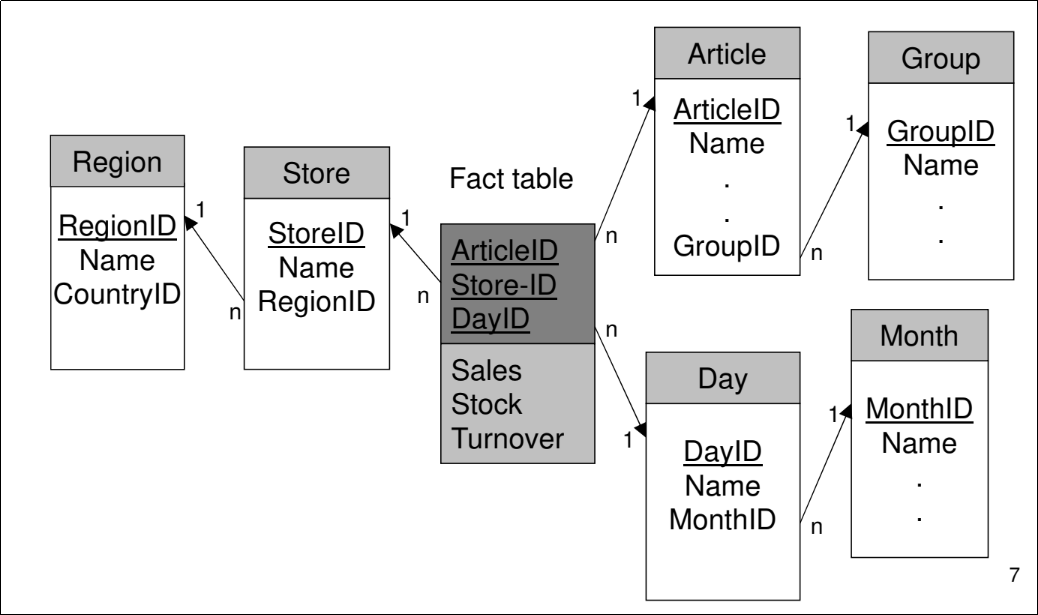
\includegraphics[width=0.8\textwidth]{snowflake.png}
    \caption{An example of a snowflake schema (the 7 is a page number)}
    \label{fig:snowflake}
\end{figure}

\subsubsection{Star Schema}
The star schema is basically a snowflake schema that is not normalized.
The data in the dimension tables is potentially very redundant, which can lead to increased memory consumption.
The joins in the query are faster (because there are fewer) with the star schema.
An example is shown in \Cref{fig:star}.

\begin{figure}[h]
    \centering
    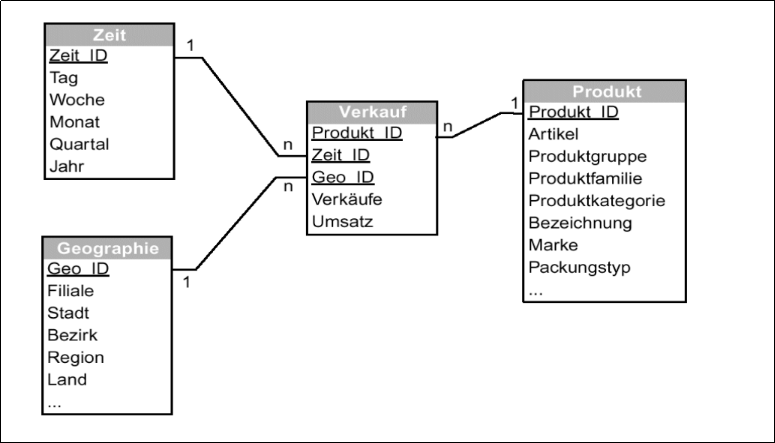
\includegraphics[width=0.8\textwidth]{star.png}
    \caption{An example of the star schema}
    \label{fig:star}
\end{figure}

\begin{keypointbox}
    If multiple cubes are necessary, just reuse and combine parts you already have.
    This leads to a galaxy representation
\end{keypointbox}

\subsection{MD Queries}
A common pattern is the star join pattern.
You simply join the fact table with the dimension table through the indices stored in the fact table.
Because grouping along multiple dimensions is a frequent use-case in DWs, modern DBMSs have special methods for that.
I will explain them in the order that I found easiest to understand.
All of this can be done with simple group by clauses and unions, but that is an absolute nightmare for larger numbers of tables, and should be avoided where possible.

\subsubsection{Grouping Sets}
A grouping set is used in the \lstinline{GROUP BY} clause of a query.
It is a set of sets defining the different groupings.
\Cref{fig:groupingset} shows a very good example of how they work (for anyone interested it was taken from the postgresql manual on grouping sets).

\begin{figure}[h]
    \centering
    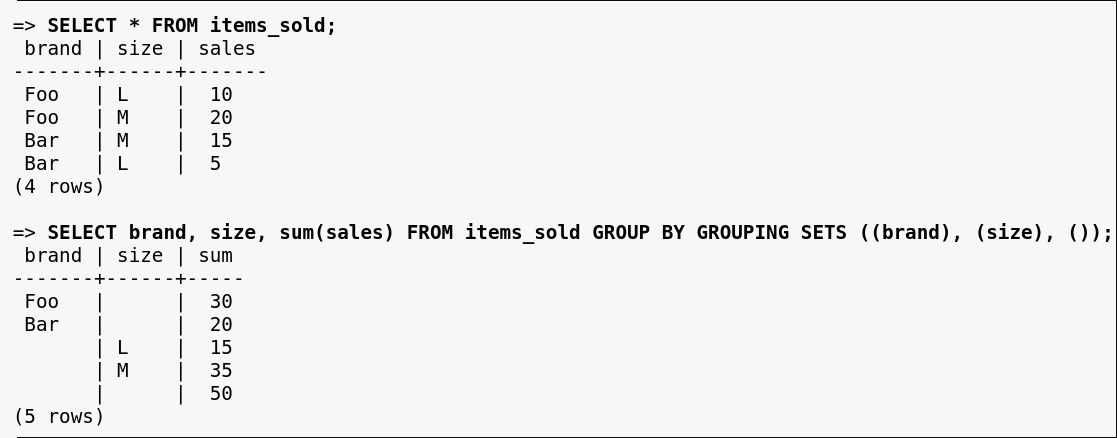
\includegraphics[width=\textwidth]{groupingset.png}
    \caption{An example of grouping sets}
    \label{fig:groupingset}
\end{figure}

\begin{keypointbox}
    A grouping set of $((a),(b,c),())$ will aggregate over rows with the same value in column $a$, then over all rows with identical $b$ and $c$ columns, and then over all.
    It will display all results in the same table.
\end{keypointbox}

\subsubsection{Rollup}
A rollup of $(a,b,c)$ is equivalent to a grouping set of $((a,b,c), (a,b), (a), ())$.
The rollup operator always adds the aggregate over all rows.
If this is not desired, the row should be filtered.

\subsubsection{Cube}
The cube operator calculates the power set of the supplied column set, and uses that as a grouping set.
For example, a cube of $(a,b,c)$ becomes a grouping set of $(a,b,c), (a,b), (a,c), (b,c), (a), (b), (c), ()$.

\begin{keypointbox}
    A \lstinline{ROLLUP} performs a rollup along a single dimension, a \lstinline{CUBE} does so along all combinations of dimensions.
\end{keypointbox}

\subsubsection{Other useful functions}
The \lstinline{GROUPING()} function tells us whether a given column was aggregated, and if multiple columns are supplied, it tells us the aggregations in a bitmask fashion.

There also usually exist nicer functions for handling date data-types.

\subsubsection{The \lstinline{OVER} Clause}
This clause allows us to include aggregations with the unaggregated data.
\Cref{fig:over} shows an example.
\lstinline{OVER} can also be used for window functions.
This is actually very well explained in the POSTGRES documentation, and a very nice example is shown in \Cref{fig:window}.
Window functions can also be used for ranking with the \lstinline{RANK()} and \lstinline{DENSE_RANK()} functions.

\begin{figure}[hp]
    \centering
    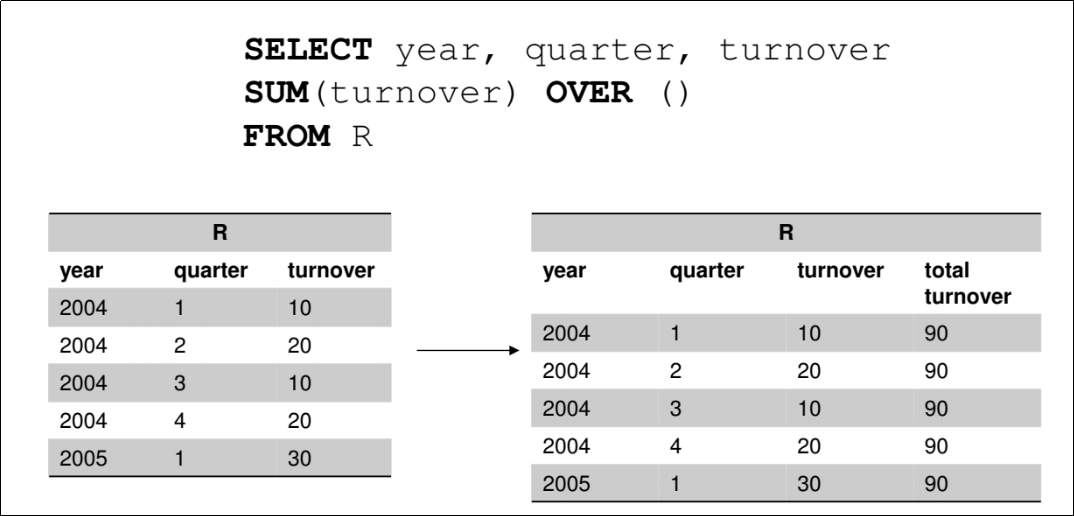
\includegraphics[width=\textwidth]{over.png}
    \caption{An example of the \lstinline{OVER} clause}
    \label{fig:over}
\end{figure}

\begin{figure}[hp]
    \centering
    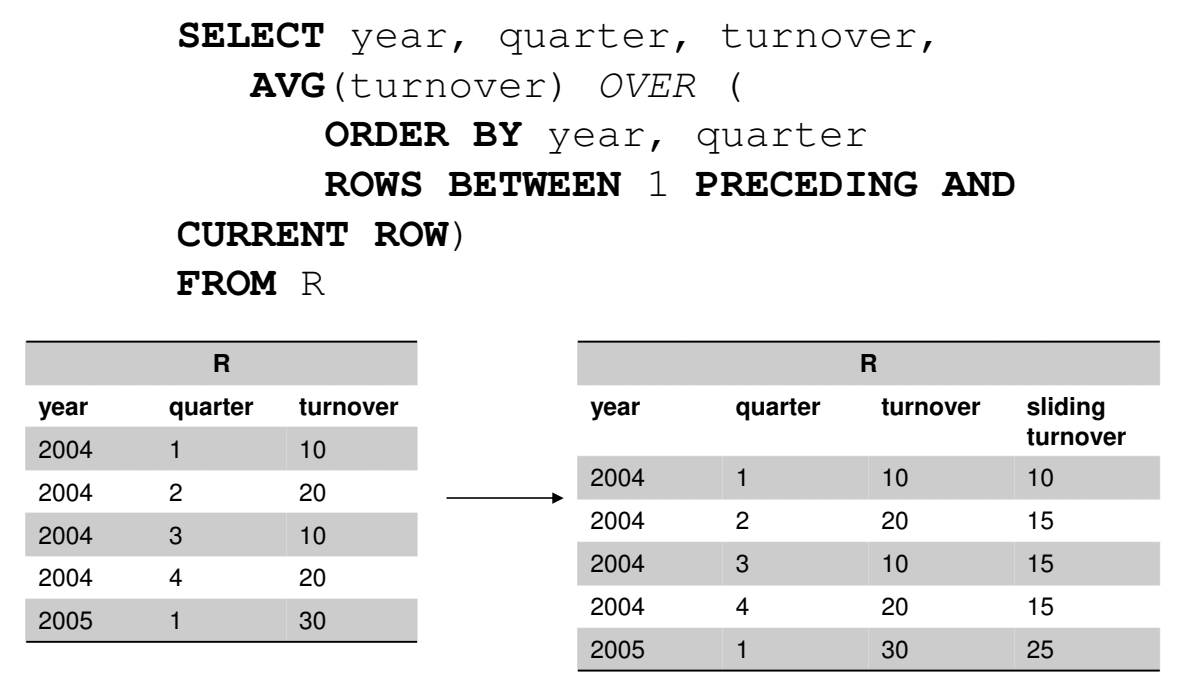
\includegraphics[width=\textwidth]{window.png}
    \caption{Using \lstinline{OVER} for sliding window computation}
    \label{fig:window}
\end{figure}

\section{Versioning}
Versioning can be very important in DWS systems.
For organizational or legal reasons, deleting entries can sometimes not be an option.
In those cases we need to add some measure of declaring a tuple invalid.

There are in general four methods of versioning:
\begin{itemize}
    \item Overwriting old values
    \item Adding a version number
    \item Tuple timestamps
    \item Attribute timestamps
\end{itemize}
Where overwriting old values leeds to data loss and is thus sometimes unacceptable.

Attribute timestamping adds a start and end validity date to every attribute (leading to non-first-normal-form tables), while timestamping saves a start and end date for every tuple.
Because we need the beginning and end time of both validity and the transaction, we need a total of four additional columns per timestamped attribute or tuple.
Adding timestamps to tuples can lead to significant memory overhead due to the redundant saving of unchanging tuple parts.

\subsection{Schema Updates}
Sometimes changes to the schema become necessary.
These are \textbf{a lot harder} to handle than instance updates, because they could force us to remodel the entire DW.
The two main methods of handling them are schema versioning and schema evolution.
For schema evolution old queries are still possible, but for a new schema this might not be the case.
The steps necessary for adapting a schema to certain changes are shown in \Cref{fig:changes}.

\begin{figure}[hp]
    \centering
    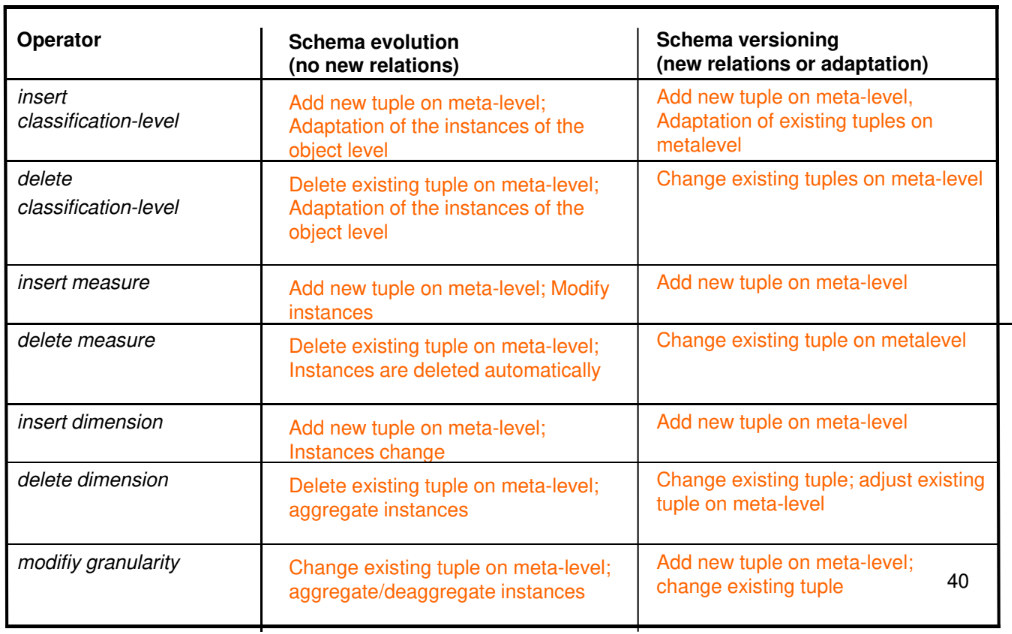
\includegraphics[width=\textwidth]{changes.png}
    \caption{Necessary steps for schema updates}
    \label{fig:changes}
\end{figure}

\section{Multi-dimensional Storage}
The best abstract model for storing things in MD fashion is a cube.
However, we do not only consider a three-dimensional cube, but an $n$ dimensional hypercube.
For visualization purposes we can reduce it to three dimensions, and our operations will work on other dimensions just the same.
We now need two (different) data structures for the dimensions (for addressing) and for the cube itself.

\subsection{Dimensions}
Abstractly viewed, a dimension is an ordered list of values (along that dimension).
These values have a fixed domain.
By ordering the dimension values we can create a mapping from dimension value to index and vice versa.
If we know all dimension values of a cell, we can then calculate its position in memory.
The order of the dimensions can be chosen arbitrarily and is fixed after setup of the data cube.
It has far reaching consequences concerning queries on the cube.

There are multiple ways for storing complex records in cubes:
\begin{itemize}
    \item \textbf{Complex cells:} These store the entire tuple of measures in the cell designated by the dimension values
    \item \textbf{Multiple cubes with flat cells:} Create one cube per measure ("Multi-Cube" approach)
    \item \textbf{Measure dimension:} Push (some) measures into the dimensions, requires all measures to be of the same data type
\end{itemize}

While single cube approaches are easier to understand, they can create large memory overhead because of large areas (volumes) in the cube with NULL values.
Multi-cube approaches limit this memory consumption, but require joins for data consolidation.

\subsection{Classification Hierachies and Aggregations}
An optimization approach is to store both the dimension values and all nodes of higher classification levels in the cube.
This means that all cells in a certain category are aggregated (for example during updates) and this aggregation is also stored in the cube, reducing the query time for future aggregations.
Such aggregations can also be done only for parts of the cube.

Unfortunately, this increases the size of the cube, which may or may not be an issue.
For small cubes it is better to just calculate these aggrgations at query time, while for larger cubes this can become vital.
Storing aggregations only for some hierarchy levels (e.g. every second) can create an optimal middle ground between both approaches.

\subsection{Partial and Virtual Cubes}
Query results for all queries on a cube are also cubes, thus allowing the same optimizations and techniques.
Also, views created on the cube are themselves (virtual) cubes and allow for the same processing as real cubes.

\subsection{Storing MD-data in MD-arrays}
A more direct approach to saving MD-data is saving them in arrays.
For any amount of dimensions we need to linearize the data for storage.
This makes storage very compact, compared to tables.
A large part of the performance stems from the order the dimensions are linearized in.
\Cref{fig:linearization} shows an example of such a linearization.

\begin{figure}[h]
    \centering
    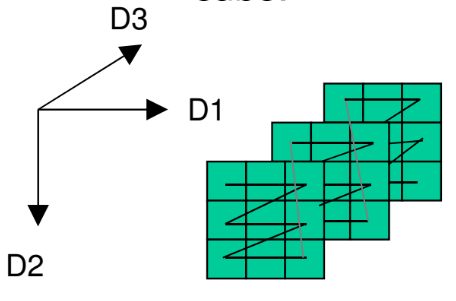
\includegraphics[width=0.4\textwidth]{linearization.png}
    \caption{An example of MD-array linearization}
    \label{fig:linearization}
\end{figure}

Calculating the index based on the dimension values is then very simple and follows the formula:
\begin{equation}
    I = \sum_{i=1}^n v_i \prod_{j=2}^i |D_{j-1}|
\end{equation}
So for three dimensions we get $I = v_1 + v_2 \cdot |D_1| + v_3 \cdot |D_1| \cdot |D_2|$.
Index calculation can be sped up using the Horner Schema.

\subsubsection{Sparse vs Dense Population}
The filling level is given by the number of filled cells, divided by the number of total cells.
Dense population is given when the filling level is high, sparse population is given when it is low.
For dense populations, array storage is more efficient than relational storage.
For sparse populations, we can make some adjustments to the array saving method to greatly increase storage efficiency.

One method is to not store empty areas in sparsely populated arrays.
If the empty cells would occupy an entire memory block, you can just skip it.
This requires additional calculations for indices.

There is also the possibility of storing sparsely populated dimensions on another level than densely populated ones.

\subsubsection{Limitations of MD-Storage}
MD-storage methods do have some limitations.
It can be expensive to maintain the full MD-array (due to null-values), and not saving NULL areas makes it more like a relational approach.
Inserting new values can cause \textbf{a lot} of memory shifting in order to keep the order on indices consistent.
There is also no current standard for MD-storage, as opposed to SQL, and all query languages are proprietary.

\subsection{Target Figures}
Target figures can be difficult to store in MD-arrays, as they are only known in spares quality (e.g. only per store per month), and need to be filled in later.
We would however still be able to calculate with them in aggregations (e.g. prognosing yearly totals for the running year).
This requires the DW to maintain the target figures itself, often with (goal) tracking.
The target figures can also be stored along with actual measures in the cube cells.

\subsection{Access Control}
Access control is a tricky issue for OLAP systems, as we want to generate accurate reports without the user obtaining specific information he or she should not usually access.
A user can also obtain specific cell values by using tracker queries and set algebra.
An example of a tracker query is shown in \Cref{fig:tracker}.
Most systems only have a simple rights system which does not protect against tracker queries.
A possible countermeasure would be to recognize tracker queries and forbid the user from accessing the results.
This could however disrupt the workflow and make generating all desired reports impossible, due to queries resembling tracker queries by chance.

\begin{figure}[h]
    \centering
    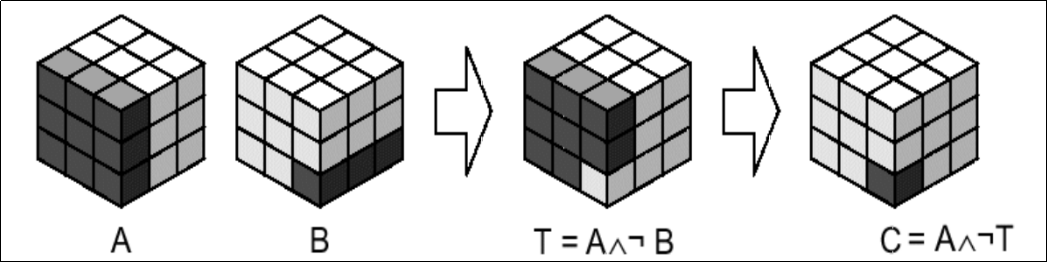
\includegraphics[width=\textwidth]{tracker.png}
    \caption{An example of tracker queries}
    \label{fig:tracker}
\end{figure}
\end{document}
